% 来源：OEBPS/Text/Section0001_split_007.xhtml#sigil_toc_id_53

\BookChapter{40}
\section[第40章\q 凯尔·巴斯：风险大师]{第40章\\ 凯尔·巴斯：风险大师}

\begin{figure}[htbp]
\centering
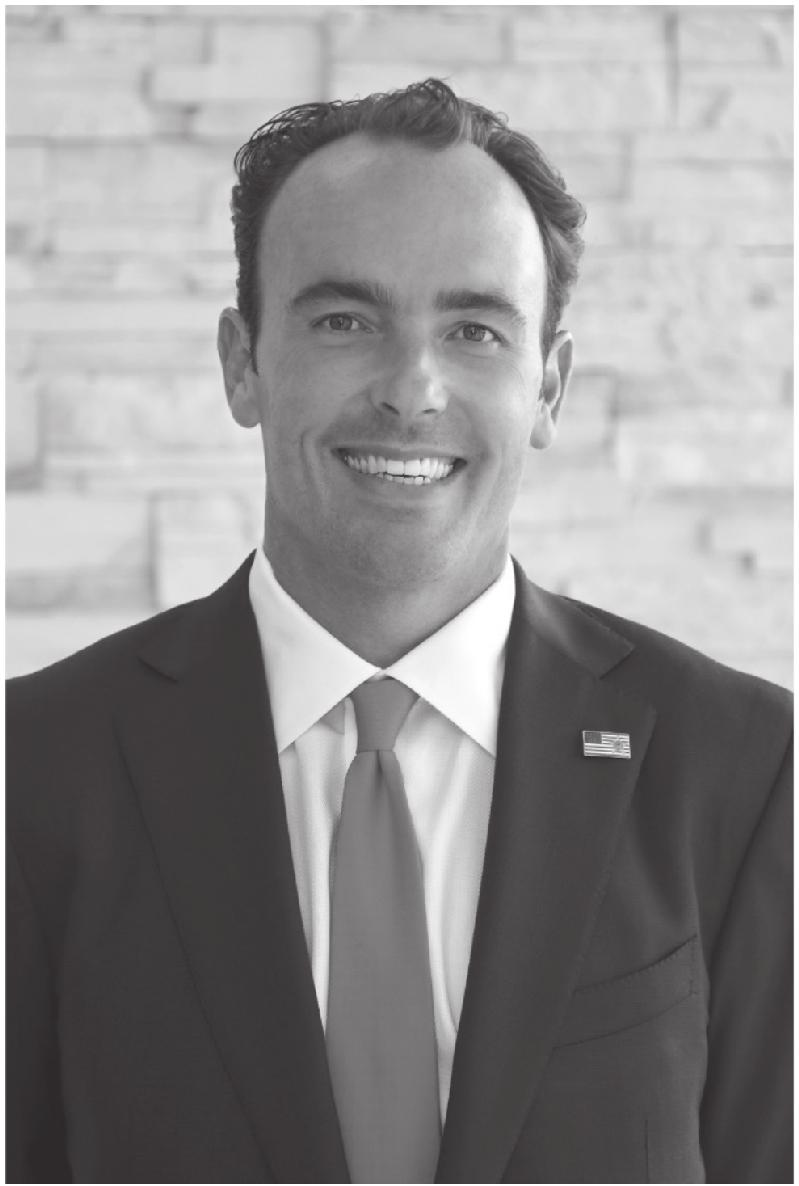
\includegraphics[width=0.40\linewidth,keepaspectratio]{image/凯尔·巴斯肖像.jpg}
\caption*{凯尔·巴斯}
\end{figure}

海曼资本管理公司创始人

凯尔·巴斯原来是一名水平很高的潜水员，他了解物理学的基本原则，他清楚地明白，涨上去的肯定还会跌下来。这正是为什么在2005年美国房地产市场一片红火时，他开始问一些别的人根本不会想更不会问的问题，例如“如果房子价格不能持续上涨（直到永远）会发生什么情况？”这些问题导致凯尔·巴斯下了世界上最大的赌注，就在2008年美国房地产即将崩溃并导致经济崩溃之前。这笔交易让凯尔·巴斯赚到了人生第一个10亿美元。凯尔·巴斯后来仅在18个月里就达到600\%的投资收益率，这让他在业内牢牢树立了自己的地位，成了当代最聪明又最具头脑的对冲基金经理。

凯尔很少接受采访，但是，他还在读大学的时候恰巧读到过我的书，那本书启发了他，所以他愿意接受我的采访。我很荣幸能飞到得克萨斯州，和他面对面交流。我们俩坐在他的办公室里，那是一栋摩天大楼，能俯视达拉斯这个伟大的城市。凯尔·巴斯是少数特立独行的金融大腕儿，认为远离美国金融中心纽约反而会给他带来竞争优势。“我们不愿意让那些噪声淹没掉。”他说。

凯尔·巴斯为人很低调，很谦卑，也很平易近人。我问他，他提出什么样的问题，导致他敢于对赌当时非常火爆的房地产市场。凯尔·巴斯回答说：“托尼，这东西又不是什么火箭科学，这只不过是个达拉斯的傻瓜问的问题罢了。”

凯尔·巴斯跟他太太、孩子生活在一起，他在得克萨斯大学投资管理公司的理事会工作，帮助监管美国最大的公共捐赠基金，资产规模超过260亿美元。你可能还记得，我在本书前面讲过凯尔·巴斯投资5美分硬币的故事，这个家伙教他的儿子学习理解风险—收益不对称，使用的方法就是购买市场价值200万美元的5美分硬币，结果他儿子第一天投资就赚了25\%。事实上，凯尔·巴斯说了，他愿意把所有的个人财富都拿来买5美分硬币，只要他在市场上能找到这么多的5美分硬币，他肯定全部买下。

除了5美分硬币之外，凯尔·巴斯一直在极其专注地寻找更多更大的风险—收益不对称的投资机会，这让他下了最近100年来两个赚钱最多的赌注：第一次是赌美国房地产市场崩盘，第二次是赌2008年开始的欧洲债务危机。凯尔·巴斯说他正在做第三次大赌，这次规模更大。我们俩在凯尔·巴斯的办公室里谈了两个半小时，下面是内容节选：

\begin{BookQuote}
\textbf{罗宾斯：}能给我们简单介绍一下你自己吗？
\end{BookQuote}

\begin{BookQuote}
\textbf{凯尔·巴斯：}我原来是一名跳水运动员，跳板跳水和高台跳水。大家都觉得跳水主要是身体上的运动，但是其实90\%是脑子里的活动，基本上就是你和你自己在脑子里做斗争。跳水让我受益匪浅。因为跳水教会了我如何用纪律约束自己，如何从失败中学习。其实，如何来对待失败决定了你是个什么样的人。我有一对非常慈爱的父母，但是我父母从来没有存过钱。我发誓我绝对不会像他们俩那样把钱全部花光，一分不留。我父母都抽烟，我发誓我绝对不抽烟。我觉得，更能驱动我的都是那些负面因素，而不是正面因素。我的人生经历，有很多地方，和你的教导完全一致。
\end{BookQuote}

\begin{BookQuote}
\textbf{罗宾斯：}你说得太对了。我去寻找能让人成功的一个共同决定因素，结果发现，有个因素远远胜过教育，远远胜过天赋，那就是饥饿感。
\end{BookQuote}

\begin{BookQuote}
\textbf{凯尔·巴斯：}饥饿和痛苦。
\end{BookQuote}

\begin{BookQuote}
\textbf{罗宾斯：}饥饿来自痛苦，如果很容易得到的话，你就不会有那种饥饿、渴求得到的感觉了。
\end{BookQuote}

\begin{BookQuote}
\textbf{凯尔·巴斯：}对，你说的没错。
\end{BookQuote}

\begin{BookQuote}
\textbf{罗宾斯：}那么，是你的饥饿感驱动你创立自己的基金，那是在2006年，对吧？
\end{BookQuote}

\begin{BookQuote}
\textbf{凯尔·巴斯：}对。
\end{BookQuote}

\begin{BookQuote}
\textbf{罗宾斯：}让我感到震惊的是，你一开始创造收益的速度简直太快了。
\end{BookQuote}

\begin{BookQuote}
\textbf{凯尔·巴斯：}那是我运气好。
\end{BookQuote}

\begin{BookQuote}
\textbf{罗宾斯：}第一年你就赚到了20\%，第二年你赚了216\%，对吧？
\end{BookQuote}

\begin{BookQuote}
\textbf{凯尔·巴斯：}对。我只是碰巧比较早就预见到了房地产抵押贷款市场会发生的情况。我相信这个说法：“幸运就是有准备的人碰到了机会。”我记得我是在上大学的时候，在你写的一本书里读到了这句话。是的，我准备好了，我喜欢这样，我很幸运，在正确的时间出现在正确的地方，因为在此之前我已经把所有需要都准备好了，就在等这一刻的到来。
\end{BookQuote}

\begin{BookQuote}
\textbf{罗宾斯：}很多人都知道房地产市场有问题，但是没有人对此采取行动。那么你和他们有什么不同？是什么让你在这个板块的投资上取得成功？
\end{BookQuote}

\begin{BookQuote}
\textbf{凯尔·巴斯：}你还记得吧，那个时候钱基本上是“免费使用”。2005—2006年，你可以用LIBOR（伦敦银行同业拆借利率）加上250个基点（一个基点相当于1/1000），拿到定期贷款，这样的利率水平，实在太便宜了，任何人都可以去融资并购一家他们想要的公司，这家公司只有一点点股东权益，剩下的就是一大堆债务，所以收购成本也非常低。那个时候我正在打电话给我的好朋友兼同事艾伦·福尼尔，我们想要搞清楚，跟房地产市场对赌如何不亏钱。那些权威专家一直在说“房价增长是就业增长和收入增长的产物”，所以只要我们的收入在增长、就业在增长，房价就会持续增长下去。这种说法当然有很大缺陷。
\end{BookQuote}

\begin{BookQuote}
\textbf{罗宾斯：}是的，我们后来都明白了。
\end{BookQuote}

\begin{BookQuote}
\textbf{凯尔·巴斯：}我到美联储参加会议，那是2006年9月，他们说：“你看，凯尔，你对这方面不太了解，因为你是个新手。你要认识到，收入增长会驱动房价增长。”我一听就说：“等等，房价和收入水平中位数完美地同步增长，已经持续50年了，但是至少最近4年，房价每年增长8\%，而收入水平每年增长只有1.5\%，所以说我们现在看到房价和收入水平中位数之间有5\textasciitilde{}6个标准差\footnote{\label{fn:pdf-40-1}在金融投资领域，标准差用在投资年化收益率上来衡量投资的波动性，标准差用历史数据计算出来的结果代表历史波动性，投资者用它来估计未来预期波动性的大小。}。”要让二者重新回到同步增长的关系，要么收入增长接近35\%，要么房价下跌30\%。于是，我打电话给华尔街的那些证券公司的分析师，我说：“我想看看你的分析模型。给我看看，如果房价一年只上涨4\%、2\%、0\%，会发生什么样的情况呢？”2000年6月，假设房价持平，增长率为0\%，拥有这个分析模型的公司，华尔街的证券公司里一家也没有，竟然一家也没有。
\end{BookQuote}

\begin{BookQuote}
\textbf{罗宾斯：}你说的是真的吗？
\end{BookQuote}

\begin{BookQuote}
\textbf{凯尔·巴斯：}真的一家也没有。
\end{BookQuote}

\begin{BookQuote}
\textbf{罗宾斯：}这些家伙都是人云亦云，都是随大流。
\end{BookQuote}

\begin{BookQuote}
\textbf{凯尔·巴斯：}2006年12月，我让瑞银证券给我构建一个分析模型，假设房地产价格持平，零增长，那么瑞银证券的模型分析表明，房地产抵押贷款资产池会损失9\%。（抵押贷款资产池就是，一批房地产抵押贷款，有相似的到期日和利率，然后打包在一起，成为一个单独的资产包或证券，这就叫抵押贷款支持证券。这些抵押贷款支持证券得到了很高的信用评级，卖给投资者，卖点是有较高的预期收益率。假设房地产价格持续上涨，这个抵押贷款资产池就会给他们带来高收益。）但是如果房地产价格不上涨，或者说只是持平，那么这些抵押贷款支持证券会下跌9\%。我一看，就打电话给艾伦·福尼尔，他以前在戴维·泰珀的阿帕卢萨投资管理公司工作，我跟他说：“就是这样，我们干吧。”于是我们俩合伙成立了一系列次贷投资基金，我组建了一家公司作为一般合伙人，我将这家公司命名为艾伦·福尼尔集团，因为我和艾伦·福尼尔打了那个电话。对于我来说，那个电话就像打开了开关。
\end{BookQuote}

\begin{BookQuote}
\textbf{罗宾斯：}请问，你和艾伦·福尼尔打的那个大赌，风险—收益之比是多少？
\end{BookQuote}

\begin{BookQuote}
\textbf{凯尔·巴斯：}嗯，大致可以这样讲，我赌房价下跌，每年只要支付3\%。就是说，如果我赌1美元，房价后来上涨了，我就赌输了，可我最多只会输掉3美分！
\end{BookQuote}

\begin{BookQuote}
\textbf{罗宾斯：}太令人震惊了。也就是说你的风险，你赌房价下跌的代价，低得简直离谱。
\end{BookQuote}

\begin{BookQuote}
\textbf{凯尔·巴斯：}是的，打赌房价下跌，我的成本只有3\%。
\end{BookQuote}

\begin{BookQuote}
\textbf{罗宾斯：}这是因为每个人都觉得，房地产市场肯定会持续上涨，永远上涨下去。那么你的上行收益是多少？
\end{BookQuote}

\begin{BookQuote}
\textbf{凯尔·巴斯：}如果房价持平或者下跌，我就会赚到整整1美元。
\end{BookQuote}

\begin{BookQuote}
\textbf{罗宾斯：}也就是说，如果你赌错了，下行风险是3\%，如果你赌对了，上行收益是100\%。
\end{BookQuote}

\begin{BookQuote}
\textbf{凯尔·巴斯：}是的。我没有听那些房地产抵押贷款专家说的话，真是一件大好事。他们见到我就会说：“凯尔·巴斯，你根本不了解你正在讲的这些东西，这不是你熟悉的市场。房价下跌这样的事根本不可能会发生。”我会说：“你这样说，对于我来说并不是一个非常充分的理由。因为我在这上面已经做了很多研究，我也许并不明白你明白的每一件事。”但是我可以避免专家容易陷入的误区，只见树木，不见森林。
\end{BookQuote}

\begin{BookQuote}
\textbf{罗宾斯：}你理解了风险—收益不对称的核心。
\end{BookQuote}

\begin{BookQuote}
\textbf{凯尔·巴斯：}我听过很多这样的说法：“房价下跌这件事根本不可能发生，因为这样整个金融体系都会崩溃的。”我觉得这样的理由也站不住脚。这是一种偏见，这种正面的、乐观的偏见，我们都有，这是人类的天性。如果你不是对自己的人生充满乐观，你就不会起床干活了，对不对？我们人类都有这种积极乐观的偏见。
\end{BookQuote}

\begin{BookQuote}
\textbf{罗宾斯：}这种积极思考的人生态度，在每个地方都很有效，只有金融世界除外。
\end{BookQuote}

\begin{BookQuote}
\textbf{凯尔·巴斯：}你说得非常对。
\end{BookQuote}

\begin{BookQuote}
\textbf{罗宾斯：}更加令人震惊的是，你准确预测房地产市场崩盘之后，你又准确预测到欧洲债务危机和希腊债务危机。你是怎么做到的？我想知道你是怎么思考的，你思考时的心理状态。
\end{BookQuote}

\begin{BookQuote}
\textbf{凯尔·巴斯：}2008年年中，贝尔斯登破产之后，雷曼兄弟破产之前，我和我的团队也是坐在办公室里，我说：“好了，美国金融危机之后，就是全球金融危机，往往先是私人资产负债表出问题，然后转移到公共资产负债表上出问题。我们搞个白板，重组一下全球各个国家的公共资产负债表。我们看看欧洲，看看日本，再看看美国。我们看看那些有很多债务的国家，我们要努力搞明白。”当时我想：“如果我是美联储主席，或者是欧洲中央银行行长，我想要充分理解这个问题，我应该做什么？我要怎么做？我会先看看我们自己整个国家的资产负债表。然后我需要知道的是，我们国家的银行体系规模有多大，要和两个指标相对而言：一个是国内生产总值，另一个是政府财政收入总额。
\end{BookQuote}

\begin{BookQuote}
\textbf{罗宾斯：}很有道理。
\end{BookQuote}

\begin{BookQuote}
\textbf{凯尔·巴斯：}我们大致看了一些国家，提出问题：“银行体系规模有多大？贷款规模有多大？”然后我们努力找出这些国家里面有哪些国家会变得糟糕，然后回过来推导，美国作为一个国家来说这又会有多么糟糕。然后我让我的团队打电话给一些证券公司的研究员，搞清楚这些国家的银行体系有多大。你猜猜，在2008年年中有多少家证券公司能搞懂各个主要国家的银行体系有多大？
\end{BookQuote}

\begin{BookQuote}
\textbf{罗宾斯：}有多少家证券公司？
\end{BookQuote}

\begin{BookQuote}
\textbf{凯尔·巴斯：}零。一家也没有。我们给每家证券公司都打电话了。
\end{BookQuote}

\begin{BookQuote}
\textbf{罗宾斯：}啊！
\end{BookQuote}

\begin{BookQuote}
\textbf{凯尔·巴斯：}于是我找了大量主权国家债务白皮书，全部都读了。这些白皮书大多数关注的是新兴市场国家的债务，因为从历史来看，重组主权国家资产负债表的都是新兴市场国家。
\end{BookQuote}

\begin{BookQuote}
\textbf{罗宾斯：}发达国家只是在世界大战之后重组过资产负债表。
\end{BookQuote}

\begin{BookQuote}
\textbf{凯尔·巴斯：}对。德国和日本两个国家把大量财富投入战争，结果战败后，欠下巨额债务。胜者为王败者为寇，胜利者得到大量战利品，失败者只能投降纳贡，每一次战争都是这样，这个世界就是这样运作的。在这种情况下，这次金融危机是世界历史上和平时期积累的最大债务规模。
\end{BookQuote}

\begin{BookQuote}
\textbf{罗宾斯：}令人震惊。
\end{BookQuote}

\begin{BookQuote}
\textbf{凯尔·巴斯：}那么银行体系有多大？我们到处寻找，搜集了很多数据，然后用了两个指标来衡量相对大小：国内生产总值，政府财政收入。这是一个艰巨的学习过程，因为以前从来没有人这样做过。
\end{BookQuote}

\begin{BookQuote}
\textbf{罗宾斯：}听起来好像除了你们之外，从来没有人这样做过。
\end{BookQuote}

\begin{BookQuote}
\textbf{凯尔·巴斯：}这又不是什么火箭科学，托尼，这只是有个达拉斯的傻瓜说：“我怎么能搞懂这个问题？”我们做了研究，我画出来一些图表，我说：“把这些国家从最差到最好按顺序排列。”谁是这张表上最糟糕的国家？
\end{BookQuote}

\begin{BookQuote}
\textbf{罗宾斯：}冰岛。
\end{BookQuote}

\begin{BookQuote}
\textbf{凯尔·巴斯：}冰岛排名第一，谁排名第二呢？这又不是火箭科学，你可以猜。
\end{BookQuote}

\begin{BookQuote}
\textbf{罗宾斯：}希腊。
\end{BookQuote}

（凯尔·巴斯点头称是。）

\begin{BookQuote}
\textbf{罗宾斯：}哇，我都猜对了。
\end{BookQuote}

\begin{BookQuote}
\textbf{凯尔·巴斯：}我们做完了所有这些研究，我看着这些分析，我说：“这不可能是对的。”我跟我的团队很夸张地说：“如果这是对的，那么你们知道接下来会发生什么？”
\end{BookQuote}

\begin{BookQuote}
\textbf{罗宾斯：}你说的对。
\end{BookQuote}

\begin{BookQuote}
\textbf{凯尔·巴斯：}于是我接着问：“哪里有针对冰岛和希腊的保险合同交易？”我的团队说“希腊是11个基点”。11个基点，就是0.11\%，我说：“好，我们要买10亿美元这种保险合同。”
\end{BookQuote}

\begin{BookQuote}
\textbf{罗宾斯：}哇，买这么多。
\end{BookQuote}

\begin{BookQuote}
\textbf{凯尔·巴斯：}提醒你一下，那是2008年的第三季度。
\end{BookQuote}

\begin{BookQuote}
\textbf{罗宾斯：}在那个阶段，这是灾难即将来临的不祥之兆。
\end{BookQuote}

\begin{BookQuote}
\textbf{凯尔·巴斯：}我打电话给哈佛大学的肯尼思·罗格夫教授，他根本不认识我。我说：“我花了好几个月构建了一张全世界的资产负债表，我想搞明白全世界的资产负债情况，我们构建出来的全世界资产负债的结果，让我觉得情况实在太糟糕了。”我急切地说，“我想，我肯定是有什么地方搞错了。请问，我可不可以去拜访您，请您看看我们的研究成果？”他说：“非常欢迎，你一定要来。”
\end{BookQuote}

\begin{BookQuote}
\textbf{罗宾斯：}太好了。
\end{BookQuote}

\begin{BookQuote}
\textbf{凯尔·巴斯：}2009年1月，我去拜访肯尼思·罗格夫教授，我们俩谈了两个半小时。我永远不会忘记那一幕：他，直奔数据分析汇总那一页，上面有张图表，汇合了所有数据，看完之后，他往椅子后面一坐，一手举起眼镜，说道：“凯尔·巴斯，我简直不敢相信，全球资产负债情况会是这么糟糕。”我一听心里马上大叫一声：“哦，天哪，我所有的担忧都得到证实了，这个人可是主权国家资产负债表分析之父啊。”很明显，如果他都没有想到过会有这种情况，那美联储主席和欧洲央行行长会想到吗？没有人想过这件事，更没有一个周密的应对计划。
\end{BookQuote}

\begin{BookQuote}
\textbf{罗宾斯：}根本没有？
\end{BookQuote}

\begin{BookQuote}
\textbf{凯尔·巴斯：}美联储主席和欧洲央行行长正在处理政府抛给他们的那些难题呢。
\end{BookQuote}

\begin{BookQuote}
\textbf{罗宾斯：}这简直令人难以相信。我得问问日本的情况，因为我知道现在你关注的是日本。
\end{BookQuote}

\begin{BookQuote}
\textbf{凯尔·巴斯：}现在，世界上最大的投资机会是在日本，要比上次次贷危机的机会更好。时机不是那么确定，但是收益率会是次贷市场的好几倍，我相信全世界压力聚集点就在日本，你要买一类保单的话，现在（差不多）是历史上最便宜的价格水平。
\end{BookQuote}

\begin{BookQuote}
\textbf{罗宾斯：}那么，这要花你多少钱？
\end{BookQuote}

\begin{BookQuote}
\textbf{凯尔·巴斯：}你要使用期权定价模型，有两个因素要考虑：一个是无风险收益率，另一个是基础资产的波动性。所以你可以想象一下，如果火鸡也是用这个理论来评估自己的风险（被主人杀掉的风险），那么基于火鸡过去活着的所有年份的历史波动性数据，分析结果会是风险为零。
\end{BookQuote}

\begin{BookQuote}
\textbf{罗宾斯：}是的。
\end{BookQuote}

\begin{BookQuote}
\textbf{凯尔·巴斯：}在感恩节来临要吃火鸡大餐之前，火鸡的分析都是对的。
\end{BookQuote}

\begin{BookQuote}
\textbf{罗宾斯：}等到感恩节要吃火鸡大餐那一天，一切都晚了。
\end{BookQuote}

\begin{BookQuote}
\textbf{凯尔·巴斯：}你想想日本，它已经有10年在压制价格和抑制波动性。波动性很小，还不到0.5个百分点。日本的资产价格低到全世界最低的水平，无风险利率只有1‰。所以你要是询问期权的定价，公式基本上会告诉你，相当于免费。
\end{BookQuote}

\begin{BookQuote}
\textbf{罗宾斯：}对。
\end{BookQuote}

\begin{BookQuote}
\textbf{凯尔·巴斯：}如果日本的债券上升150\textasciitilde{}200个基点，就是上升1.5\%\textasciitilde{}2\%，那就完了。整个金融体系就会爆炸了，这是我的看法。
\end{BookQuote}

\begin{BookQuote}
\textbf{罗宾斯：}哦。
\end{BookQuote}

\begin{BookQuote}
\textbf{凯尔·巴斯：}但是我的理论是，我也总是跟我们基金的投资人这么说：“如果移动了200个基点，那么将来就会移动1500个基点。
\end{BookQuote}

\begin{BookQuote}
\textbf{罗宾斯：}是的。
\end{BookQuote}

\begin{BookQuote}
\textbf{凯尔·巴斯：}要么就是静静地坐着一动不动，要么就是大爆炸。
\end{BookQuote}

\begin{BookQuote}
\textbf{罗宾斯：}这些都符合你所说的“尾部风险”。请给我们讲讲什么是尾部风险，很少有投资者关注尾部风险。
\end{BookQuote}

\begin{BookQuote}
\textbf{凯尔·巴斯：}你看看我正在做的事就明白了。我每年在日本债券上要花费3\textasciitilde{}4个基点，这就相当于1\%的40\%。如果你对这种情况的潜在结果的二进制看法是对的，这些债券将会有20\%的收益率，甚至更高的收益率。所以说，我为一个期权支付的成本1\%的40\%，即4‰，可能会得到20倍的收益率。托尼，在世界历史上从来没有过定价错得这样离谱的期权。不过，这只是我的个人看法，我可能是错的。不过到现在为止，我一直是对的。
\end{BookQuote}

\begin{BookQuote}
\textbf{罗宾斯：}你可能在选择时机上是错的。
\end{BookQuote}

\begin{BookQuote}
\textbf{凯尔·巴斯：}我会告诉你是怎么回事。未来10年我可能一直都是错的，如果从现在开始10年之后我是对的，那么在它发生之前我还是有100\%的概率能赢。人们会说：“你怎么会赌这种事会发生呢？以前从来没有发生过？”我会说：“如果我给你描述我刚才所说的那种情景，你却不像我这样做，你还可能会是一个精明的受托管理人吗？忘了吧，不管你认为我的预测分析是对还是错。当我给你看成本有多低时，你怎么会还不做这种投资呢？如果你的房子所在的地区很容易着火，200年前发生过一次大火把所有东西都烧了个精光，你这个业主怎么会不给这个房子买保险？
\end{BookQuote}

\begin{BookQuote}
\textbf{罗宾斯：}我明白了，这太让我感到震惊了。那么，我要问你这个问题：你认为自己是一个愿意承受相当大风险的投资人吗？
\end{BookQuote}

\begin{BookQuote}
\textbf{凯尔·巴斯：}不是。
\end{BookQuote}

\begin{BookQuote}
\textbf{罗宾斯：}我也觉得你不是。这也正是我为什么会问你这个问题的原因。你为什么说你不是一个愿意承受风险的人？
\end{BookQuote}

\begin{BookQuote}
\textbf{凯尔·巴斯：}让我换个说法，说得更清楚一些。承受相当大的风险，意味着我们可能会亏掉所有的钱，我从来不会把自己置于这种让人一记重拳击倒输掉比赛的地步。
\end{BookQuote}

\begin{BookQuote}
\textbf{罗宾斯：}请回答我最后一个重要的问题：如果你一分钱都不能留给你的孩子，只能留给他们一个投资组合清单，或者一套投资原则，那么你会告诉你的孩子什么？
\end{BookQuote}

\begin{BookQuote}
\textbf{凯尔·巴斯：}我会给他们价值200万美元的5美分硬币，因为硬币在手，他们就什么也不用担心了。
\end{BookQuote}

\begin{BookQuote}
\textbf{罗宾斯：}你已经买了200万美元的5美分硬币了，你给孩子的投资组合已经做好了。哦，我的天，这也太疯狂了。什么东西给你带来了生活中最大的快乐？
\end{BookQuote}

\begin{BookQuote}
\textbf{凯尔·巴斯：}我的孩子们。
\end{BookQuote}

\begin{BookQuote}
\textbf{罗宾斯：}难以置信。
\end{BookQuote}

\begin{BookQuote}
\textbf{凯尔·巴斯：}我可以百分之百地肯定，孩子给我带来的快乐最大。
\end{BookQuote}

\begin{BookQuote}
\textbf{罗宾斯：}凯尔·巴斯，谢谢你，和你聊天，我太开心了，我还学到了很多东西！
\end{BookQuote}
